\documentclass[11p, titlepage]{article}

\usepackage[a4paper, portrait, margin=0.9in]{geometry}
\setlength{\parskip}{1em}

\usepackage[hidelinks]{hyperref}

\usepackage{graphicx}
\graphicspath{ {./images/} }
\usepackage{caption}
\usepackage{subcaption}
\captionsetup[subfigure]{justification=centering}
\usepackage{wrapfig}

\title{COSC470 Research Project Report\\
\bigskip
Contour Splitting for Branching Structures in CT Image Reconstructions}
\author{Cameron Stevenson\\[0.5cm]{\small Supervisor: Ramakrishnan Mukundan}}

\begin{document}

\maketitle
\abstract{abstract text}
\tableofcontents

\section{Overview}

overview text
Example citation \cite{mackay2019robust, mukundan2016reconstruction, pan2017comparison}.
Example URL \footnote{\url{https://github.com/cstevenson3/cosc470writing/blob/main/survey.pdf}}.

\section{Introduction}

introduction text

\section{Background}

background text

\subsection{Generic Methods}

generic methods text

\subsection{Correspondence Methods}

subsection preamble text

\subsubsection{Contour Correspondence}

contour correspondence text

Example list:
\begin{itemize}
\item item1
\item item2
\item item3
\end{itemize}

\subsubsection{Point Correspondence and Triangulation}

pc and t text

\begin{figure}[h]
     \centering
     \begin{subfigure}[b]{0.2\textwidth}
         \centering
         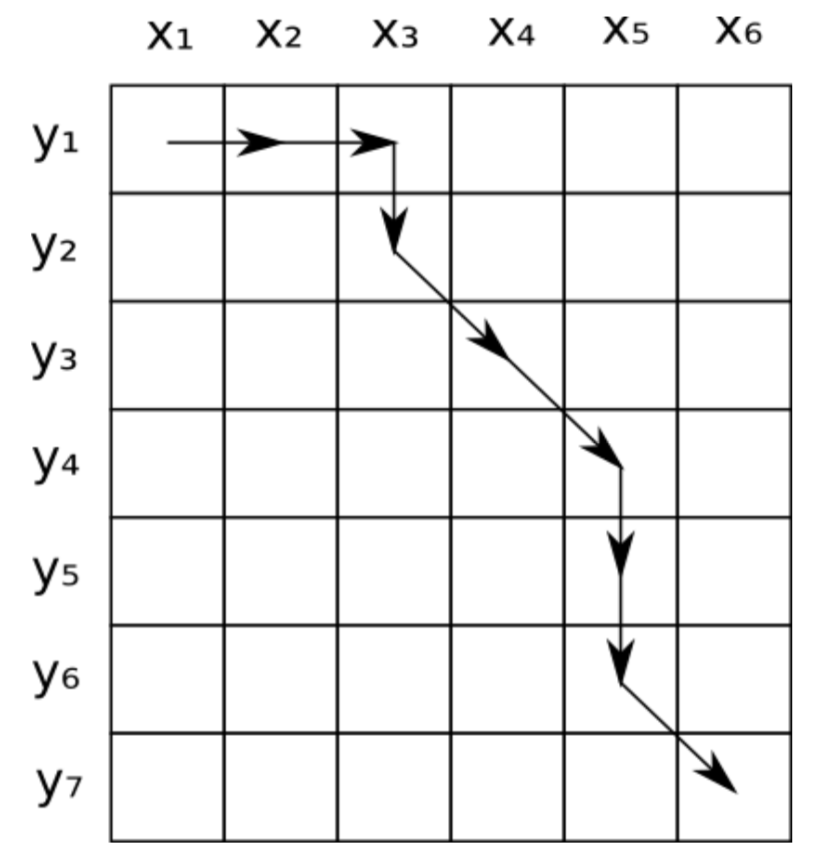
\includegraphics[width=\textwidth]{dtw1}
         \caption{DTW path through cost matrix}
         \label{fig:dtw1}
     \end{subfigure}
     \hfill
     \begin{subfigure}[b]{0.6\textwidth}
         \centering
         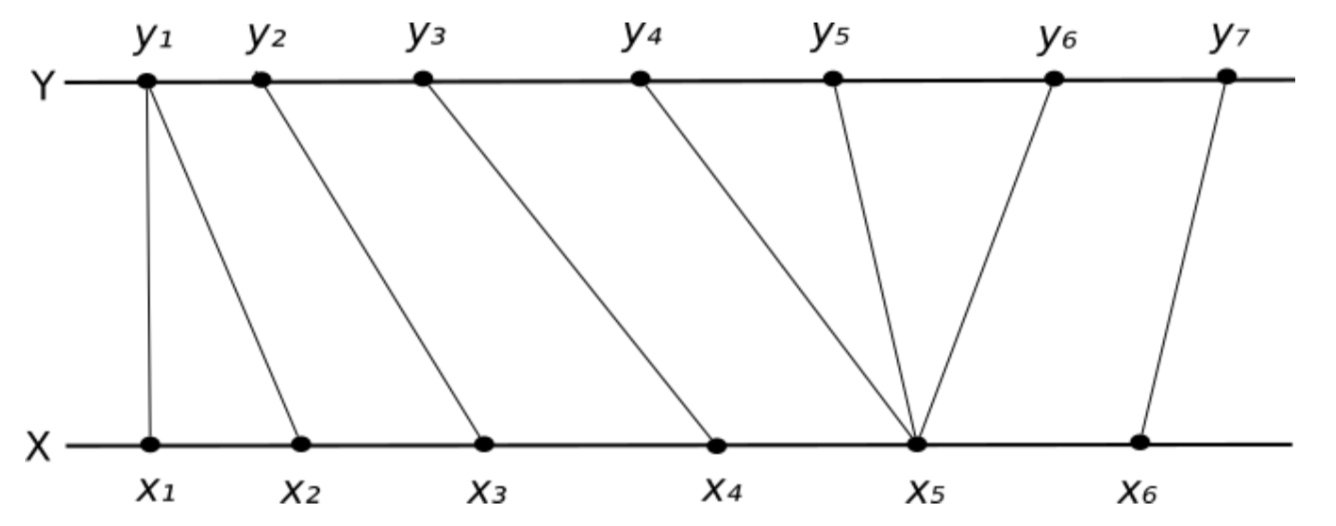
\includegraphics[width=\textwidth]{dtw2}
         \caption{DTW point correspondence}
         \label{fig:dtw2}
     \end{subfigure}
        \caption{Two examples of DTW paths on contours X and Y \cite{mackay2019robust}}
        \label{fig:dtw}
\end{figure}

text after figure declaration

\subsubsection{Branching Problem}

branching problem text

\section{Method}

method text

\subsection{Proposal}

\begin{wrapfigure}{r}{0.25\textwidth}
\centering
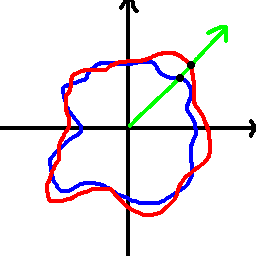
\includegraphics[width=0.2\textwidth]{pa}
\caption{Points matched by angle from shared centroid\label{fig:pa}}
\end{wrapfigure}

The proposed system consists of:
\begin{itemize}
\item Contour Splitting, a new approach to enabling point correspondence on branches and other structures
\item Point Angle, an alternative algorithm for point correspondence.
\end{itemize}

Example figure ref (See Figure \ref{fig:pa}).

\subsubsection{Contour Splitting}

For brevity, contour correspondences of 1-to-2 will be considered. Point correspondence algorithms act on 1-to-1 contour matchings, so 1-to-2 cases must be reduced to these. 

Mackay's approach was contour merging, where the 2 contour side of the correspondence is merged. The closest pair of points across the contours is found, to join them into a single contour (See Figure TODO). This gives a single 1-to-1 case for point correspondence to act on. A disadvantage of this method is that the merged contour has an unusual shape, which can cause point correspondence algorithms to behave poorly.

The proposed technique instead splits the 1 contour side of the correspondence. The best fit line to divide the 2 contour side is found, giving the angle of the line to split the 1 contour (See Figure TODO). Each half of the split 1 contour is paired with its corresponding contour on the 2 contour side. This gives two 1-to-1 cases for point correspondence to act on. The contours produced are well shaped and suitable for point correspondence algorithms designed for simpler cases.

Adjustments can be made to the position of the split line to improve accuracy. 
\begin{itemize}
\item The ratio of contour areas on the 2 contour side can be reflected in the split contour by adjusting which points the split line connects to. This preserves the internal cross section of each branch half as they join. 
\item To achieve a smooth point correspondence along the inside of the branch (where the branches join each other), the split line must have points added along it. This is in proportion to the number of points on the original contour.
\item The split line may also be adjusted in height, to reflect the likelihood the branch split is somewhere between the two planes of contours. With no further calculation, the height is assumed to be halfway. A semi-circular curve creates a split line joint which mimics the intersection of two cylinders, which is approximately what is expected from two branches coming together.
\end{itemize}

\subsection{Implementation}

pa text

\begin{figure}[h]
     \centering
     \begin{subfigure}[b]{0.22\textwidth}
         \centering
         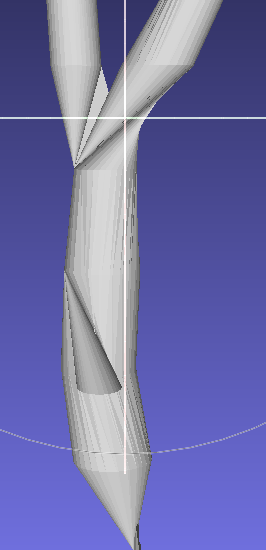
\includegraphics[width=\textwidth]{dtw10}
         \caption{DTW \linebreak}
         \label{fig:dtw10}
     \end{subfigure}
     \hfill
     \begin{subfigure}[b]{0.2\textwidth}
         \centering
         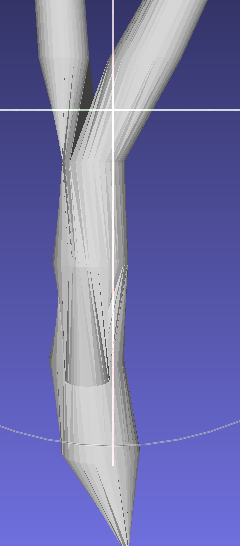
\includegraphics[width=\textwidth]{pa10ang00}
         \caption{Point angle, 0\% angle weight}
         \label{fig:pa10ang00}
     \end{subfigure}
     \hfill
     \begin{subfigure}[b]{0.195\textwidth}
         \centering
         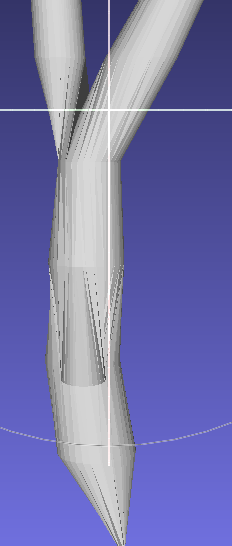
\includegraphics[width=\textwidth]{pa10ang50}
         \caption{Point angle, 50\% angle weight}
         \label{fig:pa10ang50}
     \end{subfigure}
     \hfill
     \begin{subfigure}[b]{0.2\textwidth}
         \centering
         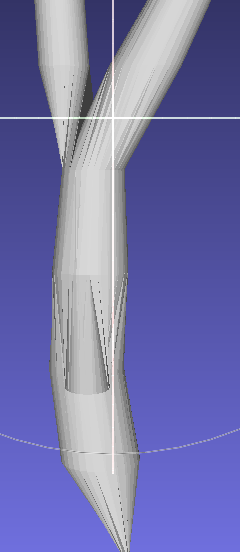
\includegraphics[width=\textwidth]{pa10ang100}
         \caption{Point angle, 100\% angle weight}
         \label{fig:pa10ang100}
     \end{subfigure}
        \caption{Reconstructions with 10 plane samples}
        \label{fig:plane10}
\end{figure}

\begin{figure}[h]
     \centering
     \begin{subfigure}[b]{0.215\textwidth}
         \centering
         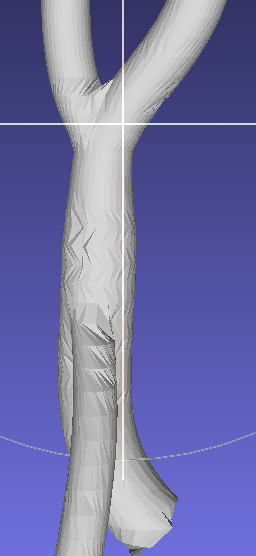
\includegraphics[width=\textwidth]{dtw50}
         \caption{DTW \linebreak}
         \label{fig:dtw50}
     \end{subfigure}
     \hfill
     \begin{subfigure}[b]{0.2\textwidth}
         \centering
         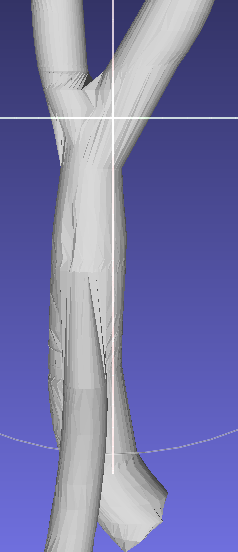
\includegraphics[width=\textwidth]{pa50ang00}
         \caption{Point angle, 0\% angle weight}
         \label{fig:pa50ang00}
     \end{subfigure}
     \hfill
     \begin{subfigure}[b]{0.205\textwidth}
         \centering
         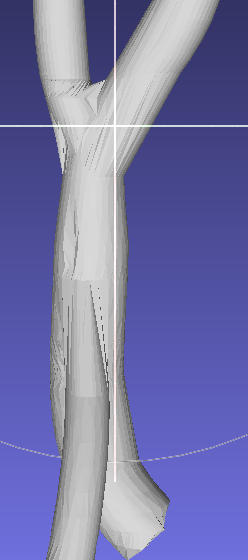
\includegraphics[width=\textwidth]{pa50ang50}
         \caption{Point angle, 50\% angle weight}
         \label{fig:pa50ang50}
     \end{subfigure}
     \hfill
     \begin{subfigure}[b]{0.2\textwidth}
         \centering
         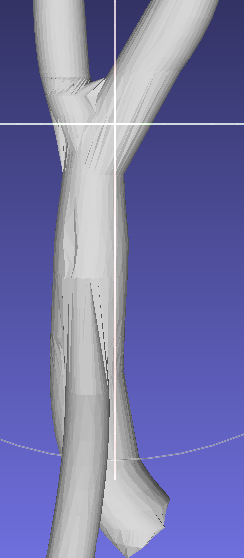
\includegraphics[width=\textwidth]{pa50ang90}
         \caption{Point angle, 90\% angle weight}
         \label{fig:pa50ang90}
     \end{subfigure}
        \caption{Reconstructions with 50 plane samples}
        \label{fig:plane50}
\end{figure}

\section{Analysis}

analysis text

\subsection{Ground Truth}

ground truth text

\subsection{Visual Results}

visual results text

\subsection{Measurements}

measurements text

\subsection{Summary}

summary text

\section{Conclusion}

conclusion text

\pagebreak
\bibliographystyle{IEEEtran}
\bibliography{references}

\section{Appendix}

\begin{figure}[h]
\centering
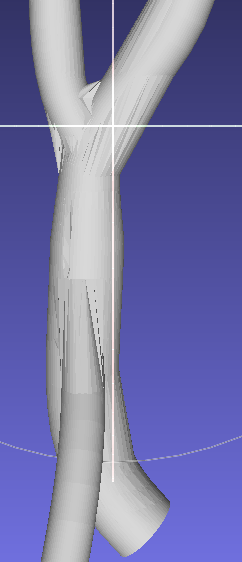
\includegraphics[width=0.29\textwidth]{mb}
\caption{Original multi branch model\label{fig:model}}
\end{figure}

\end{document}
